\documentclass[export]{beamer}

\usepackage[utf8]{inputenc}
\usepackage[T1]{fontenc}
    
\usepackage{standalone}
    
\usepackage[acronym]{glossaries}
    
\usepackage{enumitem}
    
\usepackage{xcolor}
    
\usepackage{multirow}
\usepackage{multicol}
    
\usepackage{array}
\newcolumntype{x}[1]{>{\centering\let\newline\\\arraybackslash\hspace{0pt}}p{#1}}
\usepackage{booktabs}
    
\usepackage{siunitx}
\usepackage{mathrsfs, amsmath}
    
\usepackage{graphicx}
\usepackage[font={small, color=IGNDarkGrey}, labelformat=empty]{caption}
\usepackage{subcaption}
\DeclareCaptionFont{tiny}{\tiny}
% \captionsetup[subtable]{labelfont={tiny, bf},textfont=normalfont,justification=raggedright}
% \captionsetup[subfigure]{labelfont={tiny, bf},textfont=tiny,justification=raggedright}
\usepackage{adjustbox}

\usepackage{pifont}
\newcommand{\cmark}{{\color{green} \ding{51}}}%
\newcommand{\xmark}{{\color{red} \ding{55}}}%
    
\usepackage{hyperref}
    
\usepackage[
        mcite,
        backend=bibtex,
        style=verbose,
        citestyle=authoryear,
        bibstyle=numeric,
        sorting=none,
        autocite=footnote,
        maxnames=2,
        hyperref=true,
        natbib=true,
        abbreviate=true
    ]{biblatex}
\bibliography{references}
\setbeamerfont{footnote}{size=\tiny}


\usetheme{ign}


\newacronym{acr::lod}{LoD}{Level of Detail}
\newacronym{acr::elod}{eLoD}{evalution Level of Detail}
\newacronym{acr::lidar}{LiDAR}{Light Detection and Ranging}
\newacronym{acr::dsm}{DSM}{Digital Surface Model}
\newacronym{acr::gui}{GUI}{Graphical User Interface}

\title{Semantic 3D building model evaluation}
\subtitle{}
\institute[LaSTIG STRUDEL]{Univ. Paris Est, LaSTIG STRUDEL, IGN, ENSG}
\date{\today}
\author[O.Ennafii]{Oussama Ennafii}


\begin{document}

    \begin{frame}[plain]
        \titlepage{}
    \end{frame}

    \section{Introduction}
        \subsection{Context}
        \subsection{Motivation}
        \subsection{3D Model evalutation in litterature}
            \begin{frame}[plain]{State-of-the-art illustration}
                \begin{figure}
                    \includegraphics[width=\textwidth]{state_of_the_art}
                    \caption{\label{fig::bib_summary} State of the art summary.}
                \end{figure}
            \end{frame}
        \subsection{Contributions}

    \section{Methodology}
        \begin{frame}{The evalutation pipeline}
            \begin{figure}
                \includegraphics[width=\textwidth]{graphical_abstract}
            \end{figure}
        \end{frame}

        \subsection{Error taxonomy}
            \begin{frame}{Error taxonomy summary}
                \begin{figure}
                    \includestandalone[mode=buildnew, width=\textwidth]{taxonomy_tree}
                \end{figure}
            \end{frame}
        \subsection{Extracted features}
        \subsection{Classification process}
            \begin{frame}{Classification problems summary}
                \begin{table}
                    \tiny
                    \begin{center}
                        \begin{tabular}{x{.05\textwidth} x{.06\textwidth} x{.05\textwidth} x{.7\textwidth}}
                            \toprule
                            \rotatebox{90}{\textbf{\textit{finesse}}} & \rotatebox{90}{\textbf{\acrshort{acr::elod}}} & \rotatebox{90}{\textbf{exclusivity}} & \textbf{Classification output}\\
                            \midrule
                            \scriptsize
                            \textcolor{green}{$1$} & -- & -- & Binary(Valid, Erroneous)\\
                            \textcolor{purple}{$2$} & \acrshort{acr::lod}-$1$ & -- & Binary(Valid, Building error)\\
                            \textcolor{purple}{$2$} & \acrshort{acr::lod}-$2$ & \textcolor{IGNDarkGreen}{on} & MultiClass(Valid, Building error, Facet error)\\
                            \textcolor{purple}{$2$} & \acrshort{acr::lod}-$2$ & \textcolor{red}{off} & MultiLabel(Valid, Building error, Facet error)\\
                            \textcolor{blue}{$3$} & \acrshort{acr::lod}-$1$ & \textcolor{IGNDarkGreen}{on} & MultiLabel(children(Binary(Valid, Building error)))\\
                            \textcolor{blue}{$3$} & \acrshort{acr::lod}-$2$ & \textcolor{IGNDarkGreen}{on} & MultiLabel(children(MultiClass(Valid, Building error, Facet error)))\\
                            \textcolor{blue}{$3$} & \acrshort{acr::lod}-$1$ & \textcolor{red}{off} & MultiLabel(children(Building error))\\
                            \textcolor{blue}{$3$} & \acrshort{acr::lod}-$2$ & \textcolor{red}{off} & MultiLabel(children(Building error)$\cup$ children(Facet error))\\
                            \bottomrule
                        \end{tabular}
                    \end{center}
                \end{table}
            \end{frame}

    \section{Experiments}
        \subsection{Used data}
        \subsection{Results}
        \subsection{Discussion}
            \begin{frame}{Some failure cases}
                \begin{figure}
                    \begin{center}
                    \tiny
                        \begin{tabular}{| x{.06\textwidth} | x{.035\textwidth} | x{.035\textwidth} || x{.06\textwidth} | x{.035\textwidth} | x{.035\textwidth} || x{.06\textwidth} | x{.035\textwidth} | x{.035\textwidth} || x{.06\textwidth} | x{.035\textwidth} | x{.035\textwidth} |}
                            \hline
                            \multicolumn{3}{| c ||}{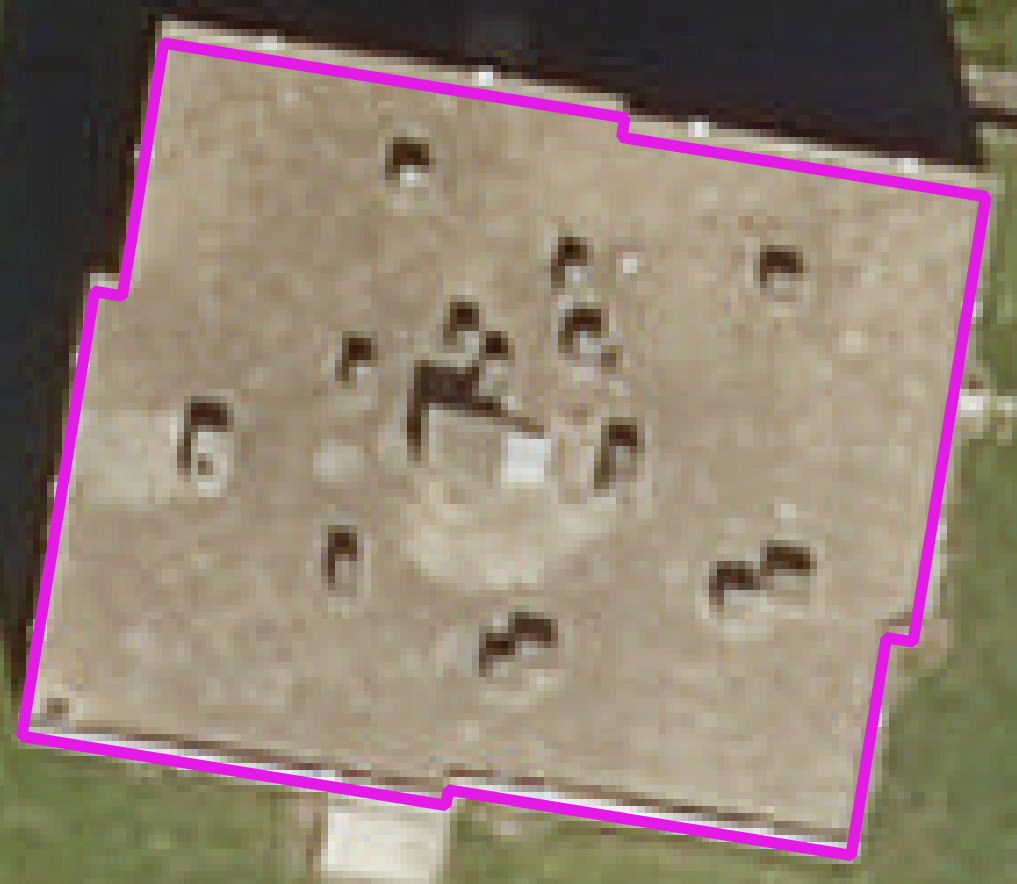
\includegraphics[width=.2\textwidth,valign=m,margin=1pt 1pt]{images/prediction_results/valid_as_bul_over}} & \multicolumn{3}{ c ||}{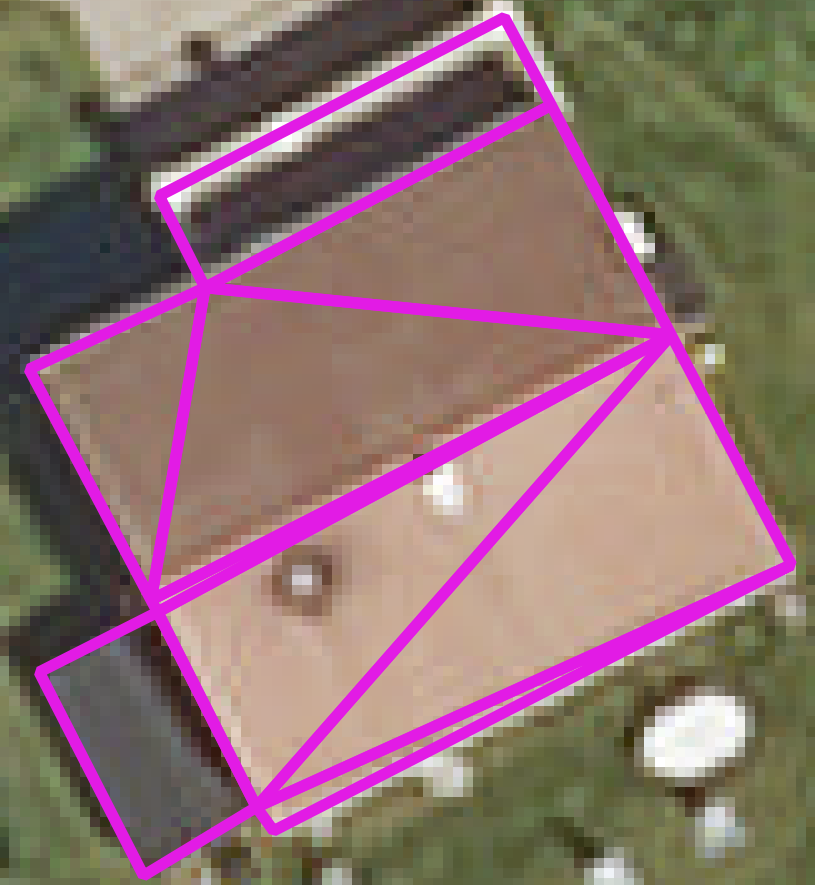
\includegraphics[width=.2\textwidth,valign=m,margin=0cm 1pt]{images/prediction_results/no_imprec_no_fac_over}} & \multicolumn{3}{ c ||}{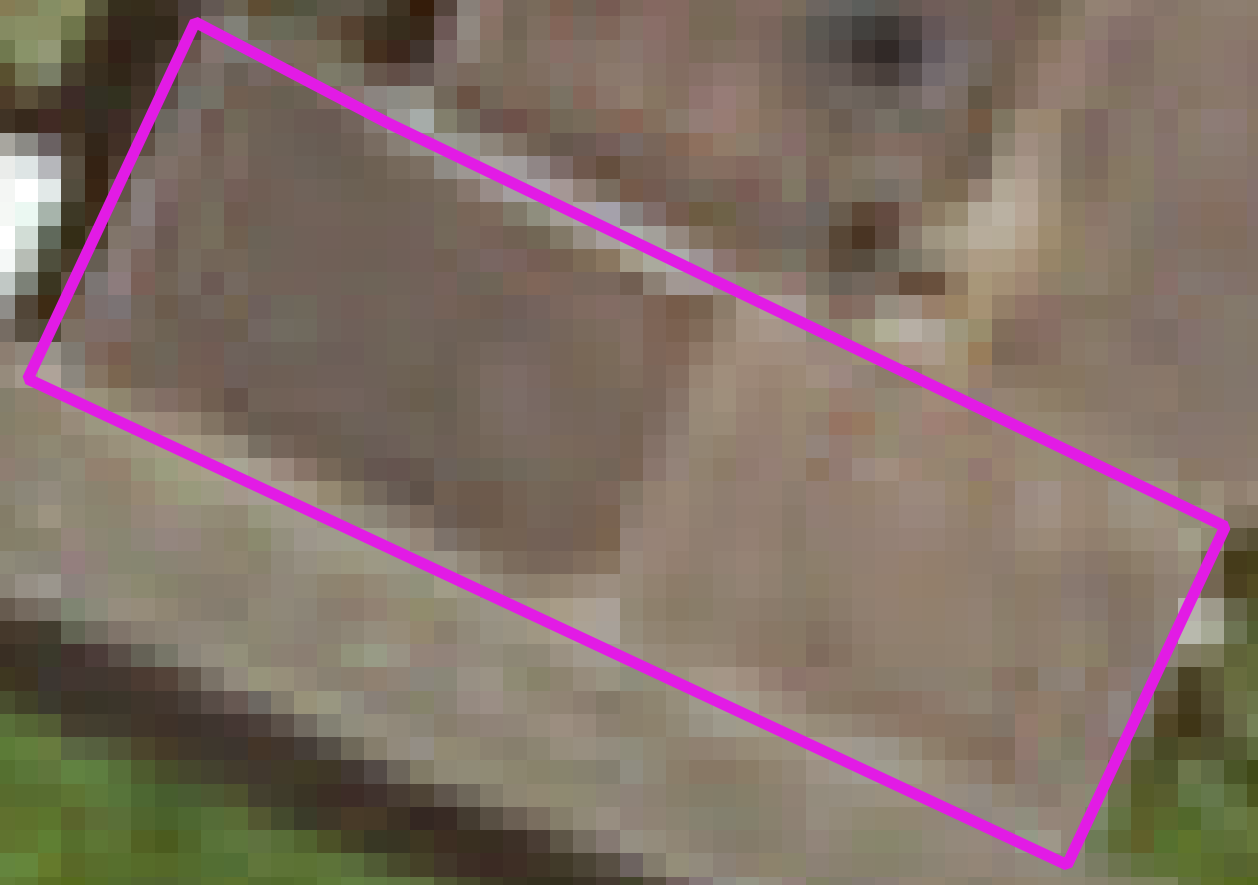
\includegraphics[width=.2\textwidth,valign=m,margin=0cm 1pt]{images/prediction_results/no_under_seg}} & \multicolumn{3}{ c |}{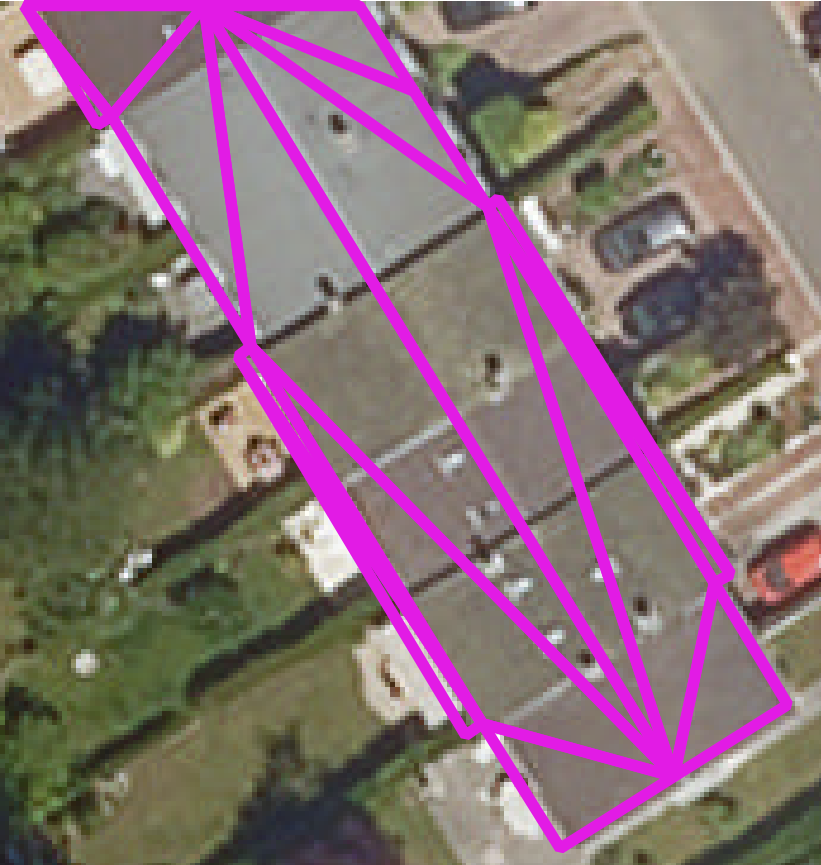
\includegraphics[width=.2\textwidth,valign=m,margin=0cm 1pt]{images/prediction_results/no_bul_under_seg}} \\
                            \hline
                            \textbf{Errors} & \textbf{G.T.} & \textbf{Pred.} & \textbf{Errors} & \textbf{G.T.} & \textbf{Pred.} & \textbf{Errors} & \textbf{G.T.} & \textbf{Pred.} & \textbf{Errors} & \textbf{G.T.} & \textbf{Pred.}\\
                            \hline
                            \textit{BOS} & \xmark & \cmark & \textit{BUS} & \xmark & \cmark & \textit{BOS} & \cmark & \cmark & \textit{BOS} & \cmark & \xmark \\
                            Valid & \cmark & \xmark & \textit{FImS} & \cmark & \xmark & \textit{FUS} & \cmark & \xmark &  \textit{FOS} & \cmark & \xmark \\
                             &  &  & \textit{FOS} & \cmark & \xmark &  &  &  & \textit{BUS} & \cmark & \xmark \\
                             &  &  &  &  &  &  &  &  &  \textit{BInF} & \cmark & \cmark \\
                            \hline
                        \end{tabular}
                    \end{center}
                \end{figure}                
            \end{frame}
    
    \section{Conclusion}
        \subsection{Percpectives}
        \subsection{Take home message}

\end{document}